\chapter{模糊数学简介}
%\author{Michal Jezewski, Robert Czabanski and Jacek Leski}
    本章主要介绍模糊集和相关的基本问题。
    第一节介绍集合讨论不同集合的概念:经典集合,模糊集,并且给出了描述模糊集的几种方法。
    第二节介绍了$t$ 形, $s$ 形,以及其他相关的模糊集形式。
    后续各节介绍了扩展原理({\it{extension principle}}),模糊关系,模糊集的合成,以及模糊集的圆柱扩展和投射. 
    第六节讨论了模糊数和他们基本的算数运算。
    最后一节总结了本章内容。
\maketitle

\section{经典集和模糊集}
经典集的概念是一个基本思想, 并无明确定义。
一般认为,一个集被认为是若干个具有一定特征区分的对象(元素)所组成的。
例如,小于100的正整数集,或者水鸟。
通常集合用大写的字母表示(如 $A, B, ...$),对象用小写字母表示(如 $x, y,...$)。
每一个集合可以被认为是宇宙域$\mathbb{X}$的子集,宇宙域可以认为是包括了所有对象的"超级集合"。

在经典集中,一个给定的对象$x$ 可以属于一个集$A$,或者不属于这个集合, 这两种运算分别被记为$x \in A$ 和 $x \notin A$。
特征函数($\chi_{A}$)可以用来描述一个经典集可以取的两个值:1(对象属于集$A$) 和 0(对象不属于集$A$).
\begin{equation}
    \chi_{A}(x)=\left\{\begin{array}{l}
    1, x \in A, \\
    0, x \notin A
    \end{array}\right.
    \end{equation}

以下给出定义在经典集上的几种基本运算:
\begin{itemize}
    \item 积(交) 
\begin{equation}
    A \cap B=\{x \in \mathbb{X} \mid x \in A \text { and } x \in B\}     
\end{equation}
    \item 和(并) 
\begin{equation}
    A \cup B=\{x \in \mathbb{X} \mid x \in A \text { or } x \in B\}
\end{equation}
    \item 非(差)
\begin{equation}
    \bar{A}=\{x \in \mathbb{X} \mid x \notin A\}
\end{equation}
\end{itemize}

以上运算在特征函数的基础上依然成立:
\begin{equation}
    \chi_{A \cap B}=\chi_{A}(x) \wedge \chi_{B}(x)=\min \left(\chi_{A}(x), \chi_{B}(x)\right) 
\end{equation}

\begin{equation}
    \chi_{A \cup B}=\chi_{A}(x) \vee \chi_{B}(x)=\max \left(\chi_{A}(x), \chi_{B}(x)\right) 
\end{equation}

\begin{equation}
\overline{\chi_{A}(x)}=1-\chi_{A}(x)
\end{equation}

\begin{figure}[htbp]
    \centering
    \begin{minipage}[t]{0.48\textwidth}
    \centering
    {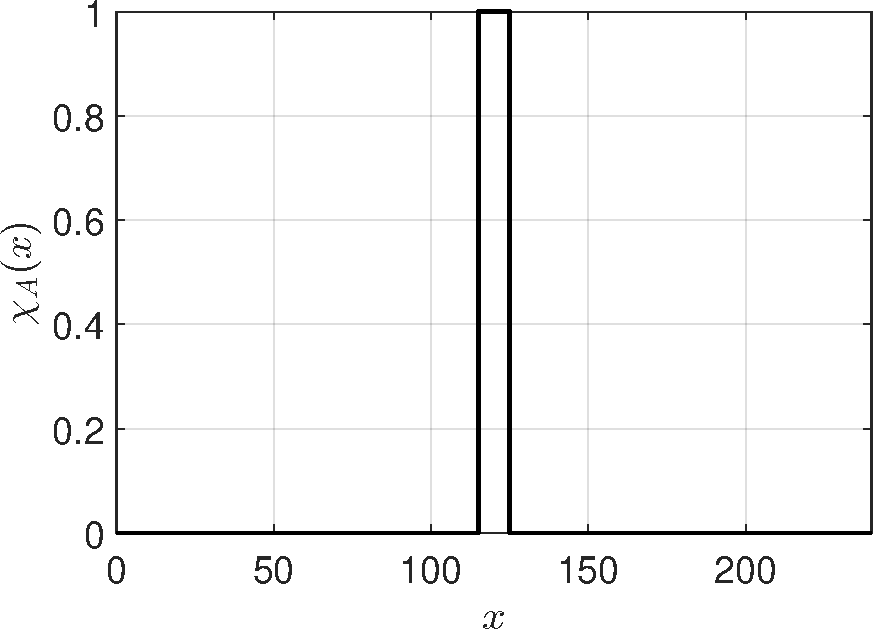
\includegraphics[width = \linewidth]{ch01/fig/heart-120.pdf}}\\ (a)
    \end{minipage}
    \hfill 
   \begin{minipage}[t]{0.48\textwidth}
    \centering
    {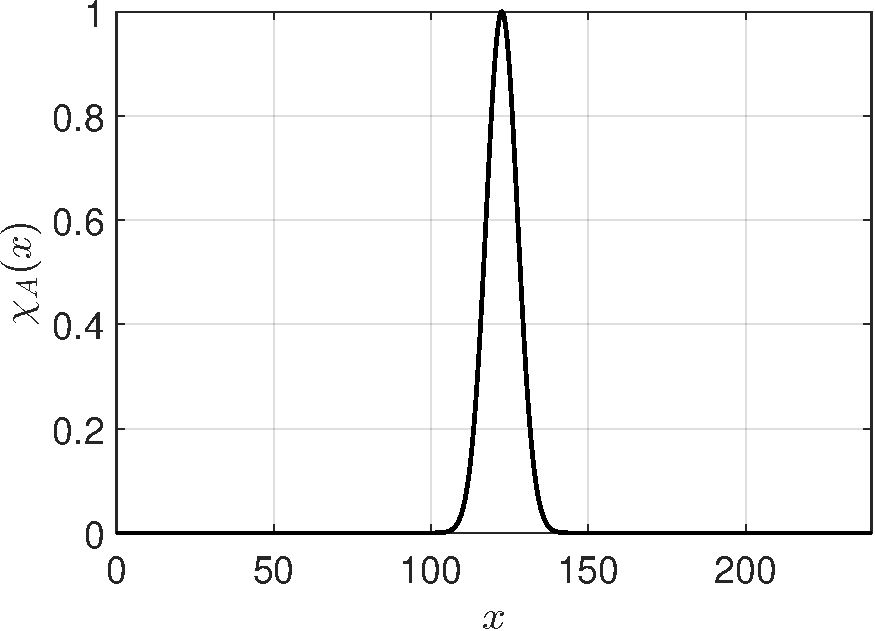
\includegraphics[width = \linewidth]{ch01/fig/heart-fuzzy.pdf}}\\ (b)
    \end{minipage}
    \caption{正常胎心率}
    \end{figure}
\begin{example}
    正常胎心率(fetal heart rate,FHR) 是 120次/分钟, 可以表示为定义在$\mathbb{X}=[0,240] \subset \mathbb{R}$上的经典集$[115,125]$。但是实验观察表明,FHR可能大于125。

    用模糊集表示

    隶属函数具有以下形式:
    \begin{itemize}
        \item 高斯型 
         \begin{equation}
            \mu_{A}(x ; c, \delta)=\exp \left(-\frac{(x-c)^{2}}{2 \delta^{2}}\right)
            \end{equation}
        \item 多项式型
        \begin{equation}
            \mu_{A}(x ; p, q, r, s)=\left\{\begin{array}{ll}
            0, & x \leq p, \\
            \frac{x-p}{q-p}, & p<x \leq q, \\
            1, & q<x \leq r, \\
            \frac{s-x}{s-r}, & r<x \leq s, \\
            0, & x>s .
            \end{array}\right.
            \end{equation}
        \item 单值型
        \begin{equation}
            \mu_{A}\left(x ; x_{0}\right)=\delta_{x, x_{0}}=\left\{\begin{array}{ll}
            1, & x=x_{0} \\
            0, & x \neq x_{0}
            \end{array}\right.
            \end{equation}  
    \end{itemize}
\end{example}
\section{模糊集的基本定义}
\section{拓展定理}
\section{模糊关系}
\section{模糊集的圆柱拓展和投射}
\section{模糊数}
\section{本章小结}